\documentclass{standalone}
\usepackage{tikz}
\usetikzlibrary{patterns, positioning}


\begin{document}
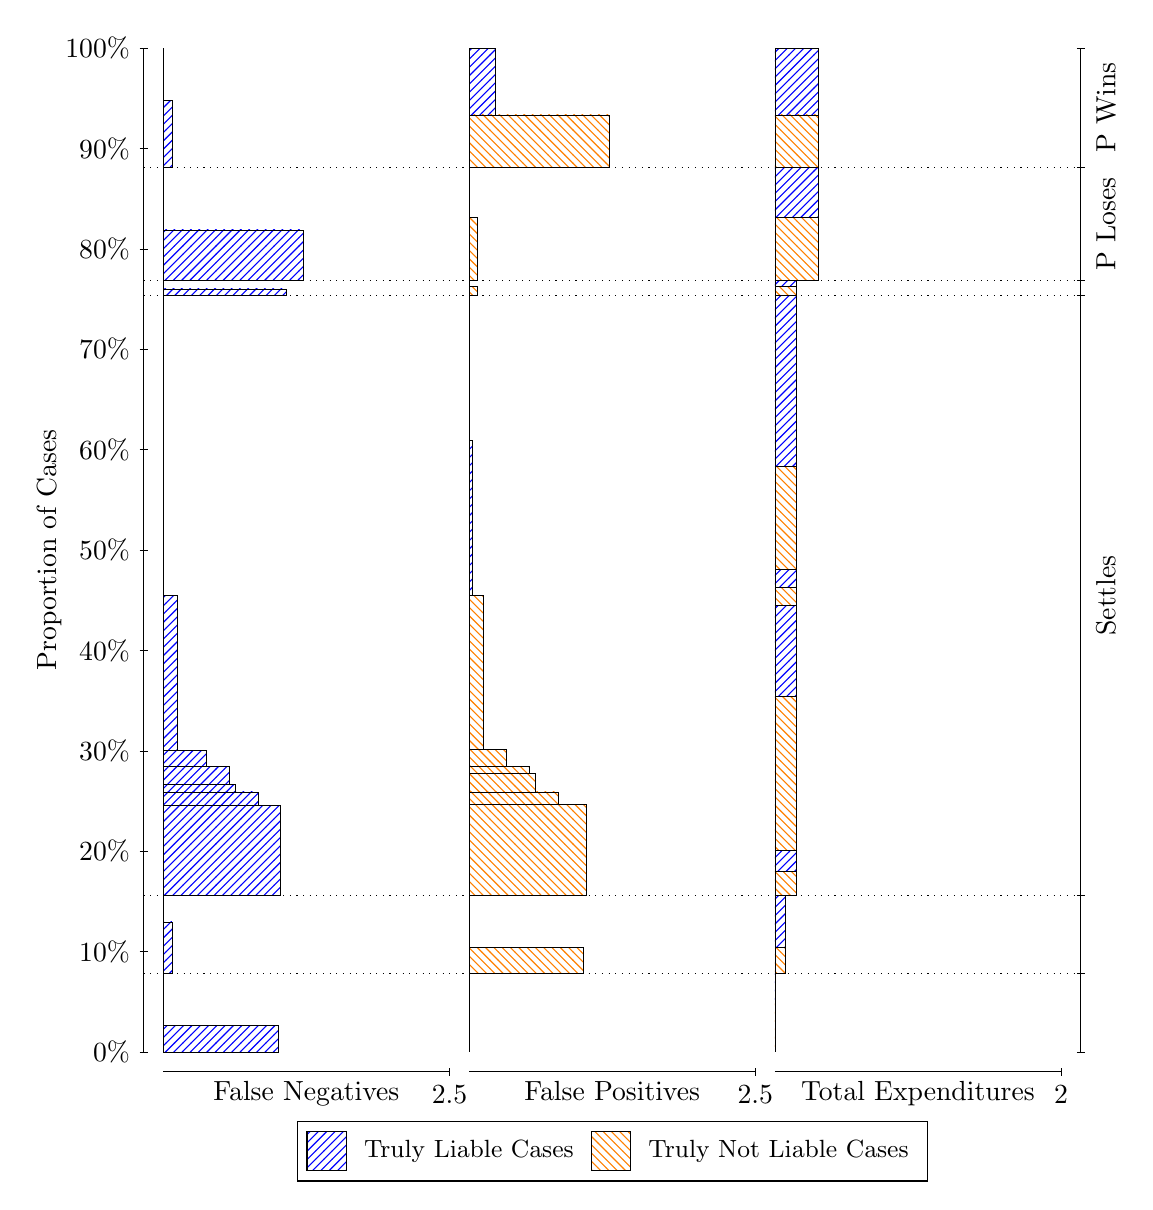
\begin{tikzpicture}
\draw[black, very thin] (1.5,1.75) -- (1.5,14.5);
\node[rotate=90, text=black, anchor=center] at (0.3, 8.125) {Proportion of Cases};
\draw[black, very thin] (1.45,1.75) -- (1.55,1.75);
\node[text=black, anchor=east] at (1.45, 1.75) {0\%};
\draw[black, very thin] (1.45,3.025) -- (1.55,3.025);
\node[text=black, anchor=east] at (1.45, 3.025) {10\%};
\draw[black, very thin] (1.45,4.3) -- (1.55,4.3);
\node[text=black, anchor=east] at (1.45, 4.3) {20\%};
\draw[black, very thin] (1.45,5.575) -- (1.55,5.575);
\node[text=black, anchor=east] at (1.45, 5.575) {30\%};
\draw[black, very thin] (1.45,6.85) -- (1.55,6.85);
\node[text=black, anchor=east] at (1.45, 6.85) {40\%};
\draw[black, very thin] (1.45,8.125) -- (1.55,8.125);
\node[text=black, anchor=east] at (1.45, 8.125) {50\%};
\draw[black, very thin] (1.45,9.4) -- (1.55,9.4);
\node[text=black, anchor=east] at (1.45, 9.4) {60\%};
\draw[black, very thin] (1.45,10.675) -- (1.55,10.675);
\node[text=black, anchor=east] at (1.45, 10.675) {70\%};
\draw[black, very thin] (1.45,11.95) -- (1.55,11.95);
\node[text=black, anchor=east] at (1.45, 11.95) {80\%};
\draw[black, very thin] (1.45,13.225) -- (1.55,13.225);
\node[text=black, anchor=east] at (1.45, 13.225) {90\%};
\draw[black, very thin] (1.45,14.5) -- (1.55,14.5);
\node[text=black, anchor=east] at (1.45, 14.5) {100\%};

\draw[black, very thin] (13.4,1.75) -- (13.4,14.5);
\draw[black, very thin] (13.35,1.75) -- (13.45,1.75);
\node[anchor=west] at (13.35, 1.75) {};
\draw[black, very thin] (13.35,2.7449) -- (13.45,2.7449);
\node[anchor=west] at (13.35, 2.7449) {};
\draw[black, very thin] (13.35,3.7383) -- (13.45,3.7383);
\node[anchor=west] at (13.35, 3.7383) {};
\draw[black, very thin] (13.35,11.358) -- (13.45,11.358);
\node[anchor=west] at (13.35, 11.358) {};
\draw[black, very thin] (13.35,11.551) -- (13.45,11.551);
\node[anchor=west] at (13.35, 11.551) {};
\draw[black, very thin] (13.35,12.984) -- (13.45,12.984);
\node[anchor=west] at (13.35, 12.984) {};
\draw[black, very thin] (13.35,14.5) -- (13.45,14.5);
\node[anchor=west] at (13.35, 14.5) {};

\draw[black, very thin, pattern color=blue, pattern=north east lines] (1.75,1.75) rectangle (3.2033,2.0858);
\draw[black, very thin, pattern color=orange, pattern=north west lines] (1.75,2.0858) rectangle (1.75,2.7449);
\draw[black, very thin, pattern color=blue, pattern=north east lines] (1.75,2.7449) rectangle (1.859,3.4033);
\draw[black, very thin, pattern color=orange, pattern=north west lines] (1.75,3.4033) rectangle (1.75,3.7383);
\draw[black, very thin, pattern color=blue, pattern=north east lines] (1.75,3.7383) rectangle (3.2397,4.8855);
\draw[black, very thin, pattern color=blue, pattern=north east lines] (1.75,4.8855) rectangle (2.949,5.0541);
\draw[black, very thin, pattern color=blue, pattern=north east lines] (1.75,5.0541) rectangle (2.6583,5.1516);
\draw[black, very thin, pattern color=blue, pattern=north east lines] (1.75,5.1516) rectangle (2.5857,5.3808);
\draw[black, very thin, pattern color=blue, pattern=north east lines] (1.75,5.3808) rectangle (2.295,5.5803);
\draw[black, very thin, pattern color=blue, pattern=north east lines] (1.75,5.5803) rectangle (1.9317,7.548);
\draw[black, very thin, pattern color=orange, pattern=north west lines] (1.75,7.548) rectangle (1.75,11.358);
\draw[black, very thin, pattern color=blue, pattern=north east lines] (1.75,11.358) rectangle (3.3123,11.44);
\draw[black, very thin, pattern color=orange, pattern=north west lines] (1.75,11.44) rectangle (1.75,11.551);
\draw[black, very thin, pattern color=blue, pattern=north east lines] (1.75,11.551) rectangle (3.5303,12.19);
\draw[black, very thin, pattern color=orange, pattern=north west lines] (1.75,12.19) rectangle (1.75,12.984);
\draw[black, very thin, pattern color=blue, pattern=north east lines] (1.75,12.984) rectangle (1.859,13.834);
\draw[black, very thin, pattern color=orange, pattern=north west lines] (1.75,13.834) rectangle (1.75,14.5);
\draw[black, very thin, pattern color=orange, pattern=north west lines] (5.6333,1.75) rectangle (5.6333,2.4091);
\draw[black, very thin, pattern color=blue, pattern=north east lines] (5.6333,2.4091) rectangle (5.6333,2.7449);
\draw[black, very thin, pattern color=orange, pattern=north west lines] (5.6333,2.7449) rectangle (7.0867,3.0799);
\draw[black, very thin, pattern color=blue, pattern=north east lines] (5.6333,3.0799) rectangle (5.6333,3.7383);
\draw[black, very thin, pattern color=orange, pattern=north west lines] (5.6333,3.7383) rectangle (7.123,4.8914);
\draw[black, very thin, pattern color=orange, pattern=north west lines] (5.6333,4.8914) rectangle (6.7597,5.0541);
\draw[black, very thin, pattern color=orange, pattern=north west lines] (5.6333,5.0541) rectangle (6.469,5.2832);
\draw[black, very thin, pattern color=orange, pattern=north west lines] (5.6333,5.2832) rectangle (6.3963,5.381);
\draw[black, very thin, pattern color=orange, pattern=north west lines] (5.6333,5.381) rectangle (6.1057,5.5888);
\draw[black, very thin, pattern color=orange, pattern=north west lines] (5.6333,5.5888) rectangle (5.815,7.5484);
\draw[black, very thin, pattern color=blue, pattern=north east lines] (5.6333,7.5484) rectangle (5.6697,9.5161);
\draw[black, very thin, pattern color=blue, pattern=north east lines] (5.6333,9.5161) rectangle (5.6333,11.358);
\draw[black, very thin, pattern color=orange, pattern=north west lines] (5.6333,11.358) rectangle (5.7423,11.469);
\draw[black, very thin, pattern color=blue, pattern=north east lines] (5.6333,11.469) rectangle (5.6333,11.551);
\draw[black, very thin, pattern color=orange, pattern=north west lines] (5.6333,11.551) rectangle (5.7423,12.345);
\draw[black, very thin, pattern color=blue, pattern=north east lines] (5.6333,12.345) rectangle (5.6333,12.984);
\draw[black, very thin, pattern color=orange, pattern=north west lines] (5.6333,12.984) rectangle (7.4137,13.65);
\draw[black, very thin, pattern color=blue, pattern=north east lines] (5.6333,13.65) rectangle (5.9603,14.5);
\draw[black, very thin, pattern color=orange, pattern=north west lines] (9.5167,1.75) rectangle (9.5167,2.4091);
\draw[black, very thin, pattern color=blue, pattern=north east lines] (9.5167,2.4091) rectangle (9.5167,2.7449);
\draw[black, very thin, pattern color=orange, pattern=north west lines] (9.5167,2.7449) rectangle (9.6529,3.0799);
\draw[black, very thin, pattern color=blue, pattern=north east lines] (9.5167,3.0799) rectangle (9.6529,3.7383);
\draw[black, very thin, pattern color=orange, pattern=north west lines] (9.5167,3.7383) rectangle (9.7892,4.044);
\draw[black, very thin, pattern color=blue, pattern=north east lines] (9.5167,4.044) rectangle (9.7892,4.3101);
\draw[black, very thin, pattern color=orange, pattern=north west lines] (9.5167,4.3101) rectangle (9.7892,6.2697);
\draw[black, very thin, pattern color=blue, pattern=north east lines] (9.5167,6.2697) rectangle (9.7892,7.4168);
\draw[black, very thin, pattern color=orange, pattern=north west lines] (9.5167,7.4168) rectangle (9.7892,7.646);
\draw[black, very thin, pattern color=blue, pattern=north east lines] (9.5167,7.646) rectangle (9.7892,7.8751);
\draw[black, very thin, pattern color=orange, pattern=north west lines] (9.5167,7.8751) rectangle (9.7892,9.1908);
\draw[black, very thin, pattern color=blue, pattern=north east lines] (9.5167,9.1908) rectangle (9.7892,11.358);
\draw[black, very thin, pattern color=orange, pattern=north west lines] (9.5167,11.358) rectangle (9.7892,11.469);
\draw[black, very thin, pattern color=blue, pattern=north east lines] (9.5167,11.469) rectangle (9.7892,11.551);
\draw[black, very thin, pattern color=orange, pattern=north west lines] (9.5167,11.551) rectangle (10.062,12.345);
\draw[black, very thin, pattern color=blue, pattern=north east lines] (9.5167,12.345) rectangle (10.062,12.984);
\draw[black, very thin, pattern color=orange, pattern=north west lines] (9.5167,12.984) rectangle (10.062,13.65);
\draw[black, very thin, pattern color=blue, pattern=north east lines] (9.5167,13.65) rectangle (10.062,14.5);
\draw[black, dotted] (1.5,2.7449) -- (13.4,2.7449);
\draw[black, dotted] (1.5,3.7383) -- (13.4,3.7383);
\draw[black, dotted] (1.5,11.358) -- (13.4,11.358);
\draw[black, dotted] (1.5,11.551) -- (13.4,11.551);
\draw[black, dotted] (1.5,12.984) -- (13.4,12.984);
\draw[black, very thin] (1.75,1.5) -- (5.3833,1.5);
\node[text=black, anchor=north] at (3.5667, 1.5) {False Negatives};
\draw[black, very thin] (5.3833,1.45) -- (5.3833,1.55);
\node[text=black, anchor=north] at (5.3833, 1.45) {2.5};

\draw[black, very thin] (5.6333,1.5) -- (9.2667,1.5);
\node[text=black, anchor=north] at (7.45, 1.5) {False Positives};
\draw[black, very thin] (9.2667,1.45) -- (9.2667,1.55);
\node[text=black, anchor=north] at (9.2667, 1.45) {2.5};

\draw[black, very thin] (9.5167,1.5) -- (13.15,1.5);
\node[text=black, anchor=north] at (11.333, 1.5) {Total Expenditures};
\draw[black, very thin] (13.15,1.45) -- (13.15,1.55);
\node[text=black, anchor=north] at (13.15, 1.45) {2};



\node[text=black, centered, rotate=90] at (13.72, 7.5482) {Settles};

\node[text=black, centered, rotate=90] at (13.72, 12.267) {P Loses};
\node[text=black, centered, rotate=90] at (13.72, 13.742) {P Wins};

\draw (7.449999999999999,1.5) node[draw=none] (baseCoordinate) {};
\begin{scope}[align=center]
        \matrix[scale=0.5, draw=black, below=0.5cm of baseCoordinate, nodes={draw}, column sep=0.1cm]{
            \node[rectangle, draw, minimum width=0.5cm, minimum height=0.5cm, pattern color=blue, pattern=north east lines] {}; &
            \node[draw=none, font=\small, text=black] (B) {Truly Liable Cases}; &
            \node[rectangle, draw, minimum width=0.5cm, minimum height=0.5cm, pattern color=orange, pattern=north west lines] {}; &
            \node[draw=none, font=\small, text=black] (B) {Truly Not Liable Cases}; \\
            };
\end{scope}

\end{tikzpicture}
\end{document}